\documentclass{article}
\usepackage{arxiv}
\usepackage[utf8]{inputenc} % allow utf-8 input
\usepackage[T1]{fontenc}    % use 8-bit T1 fonts
\usepackage{hyperref}       % hyperlinks
\usepackage{url}            % simple URL typesetting
\usepackage{booktabs}       % professional-quality tables
\usepackage{amsfonts}       % blackboard math symbols
\usepackage{nicefrac}       % compact symbols for 1/2, etc.
\usepackage{microtype}      % microtypography
\usepackage{lipsum}
\usepackage{upgreek}
\usepackage{graphicx}
\usepackage[version=4]{mhchem}
\usepackage{gensymb}
\usepackage{verbatim}
\usepackage{amsmath}
\usepackage{amssymb}

\title{Carbon cathodes for rechargeable aluminium-ion batteries}
\author{
Shalini Divya\\
  School of Chemical and Physial Sciences\\
  Victoria University of Wellington\\
  Wellington, New Zealand\\
  \texttt{shalini.divya@vuw.ac.nz}\\
  %% examples of more authors
   \And
  Thomas Nann\thanks{Corresponding author.}\\
  School of Mathematical and Chemical Sciences\\
  The University of Newcastle\\
  Newcastle, NSW 2308, Australia\\
  \texttt{thomas.nann@newcastle.edu.au}\\
}


\begin{document}
\maketitle
\section*{Supporting Information}
\newcommand{\beginsupplement}{
               \setcounter{figure}{0}
        \renewcommand{\thefigure}{S\arabic{figure}}
     }
\beginsupplement


\begin{figure}[ht!]
\centering
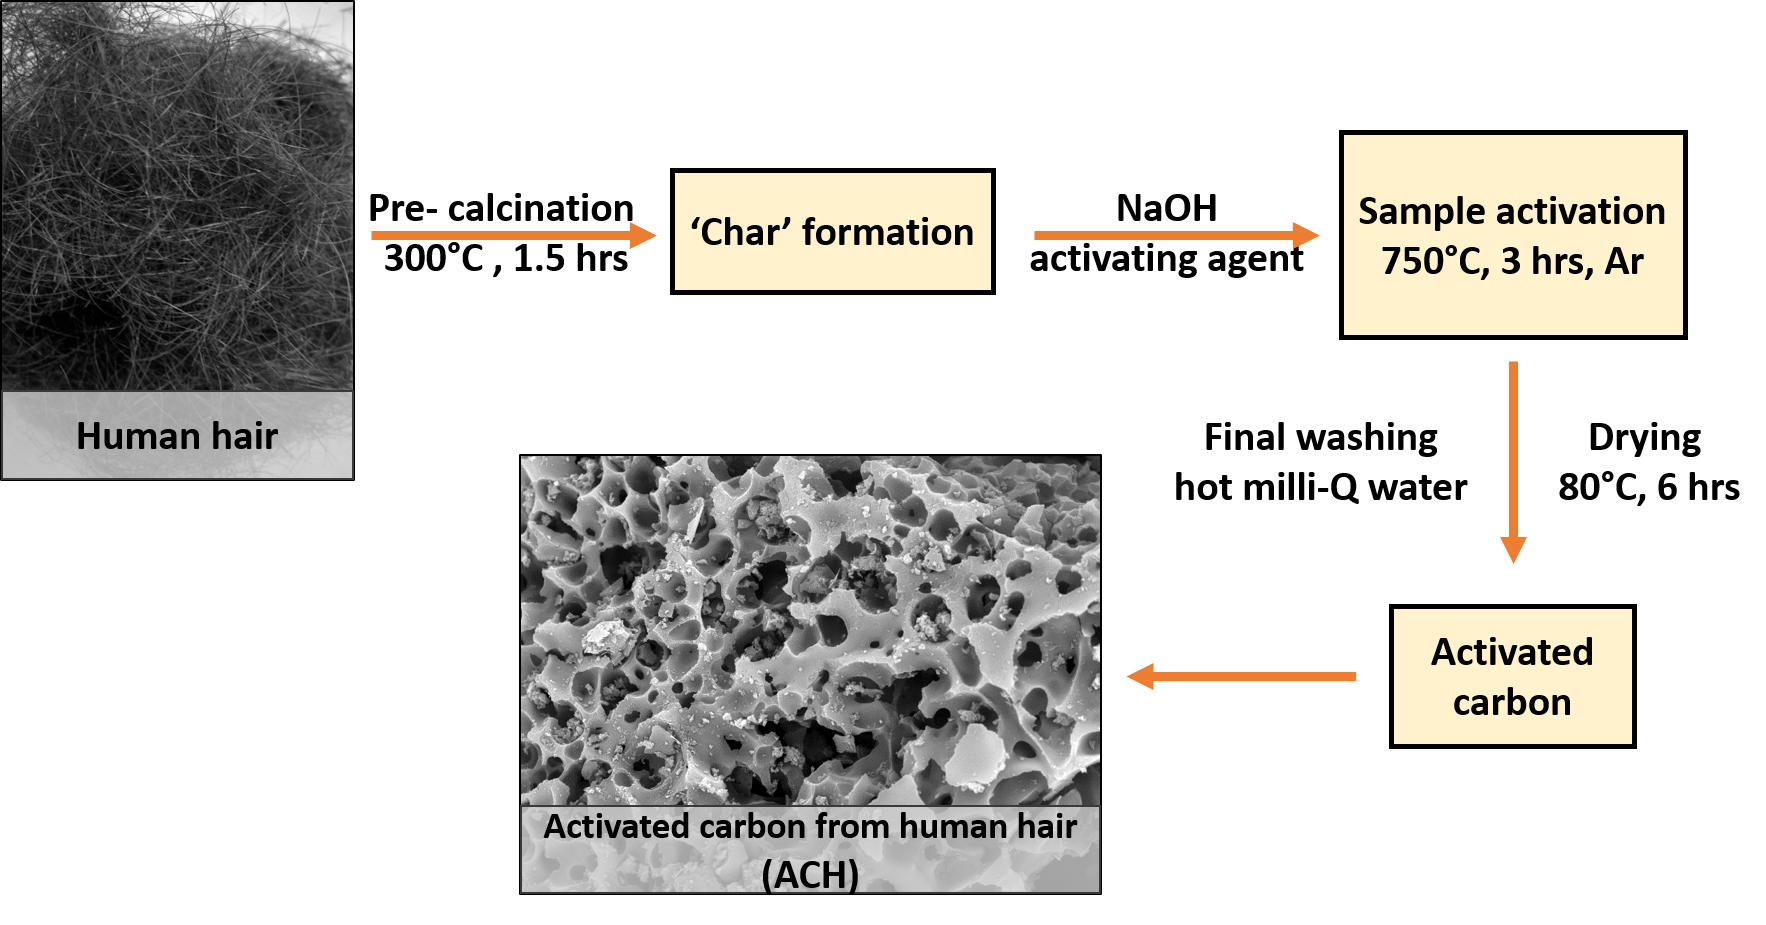
\includegraphics[width=\textwidth]{fig/ACHsyn}
\caption{Synthesis of activated carbon from human hair using NaOH as the activating agent.}
\label{fig:ACHsyn}
\end{figure}

\begin{figure}[th!]
\centering
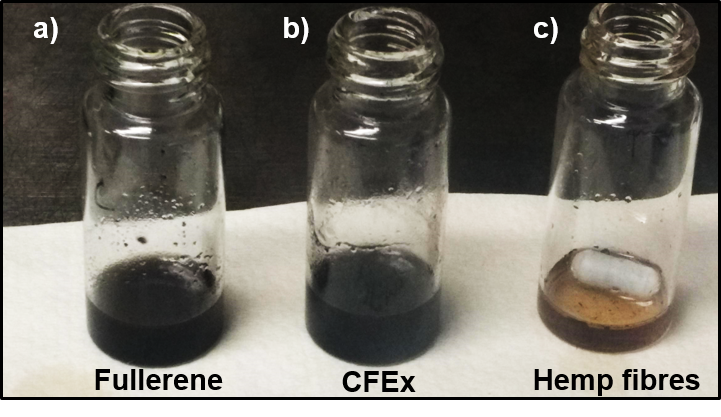
\includegraphics[width=\textwidth]{fig/CFExsol}
\caption{Synthesis of activated carbon from human hair using NaOH as the activating agent. The choice of temperature and activating agent plays a crucial role in determining pore size of the activated carbon.}
\label{fig:CFExsol}
\end{figure}

\begin{figure}[th!]
\centering
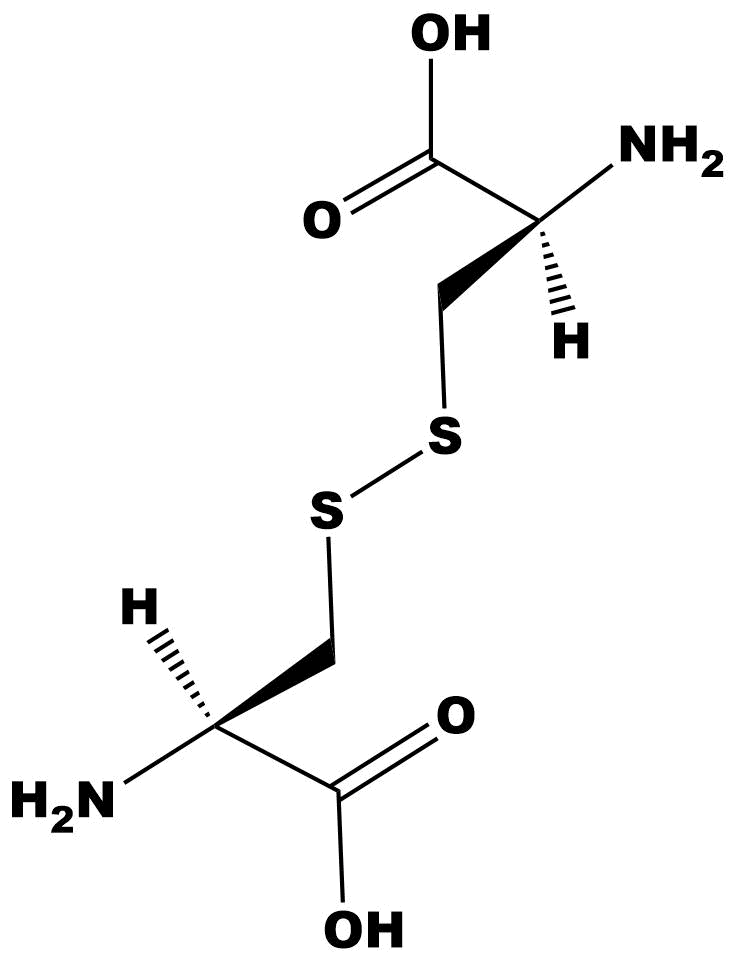
\includegraphics[width=0.5\textwidth]{fig/keratin}
\caption{Keratin: a protein abundantly found in human hair contains C-O, C=O, C-NH$_2$ bonds.}
\label{fig:keratin}
\end{figure}
%\begin{figure}[tbh!]
  %\centering
  %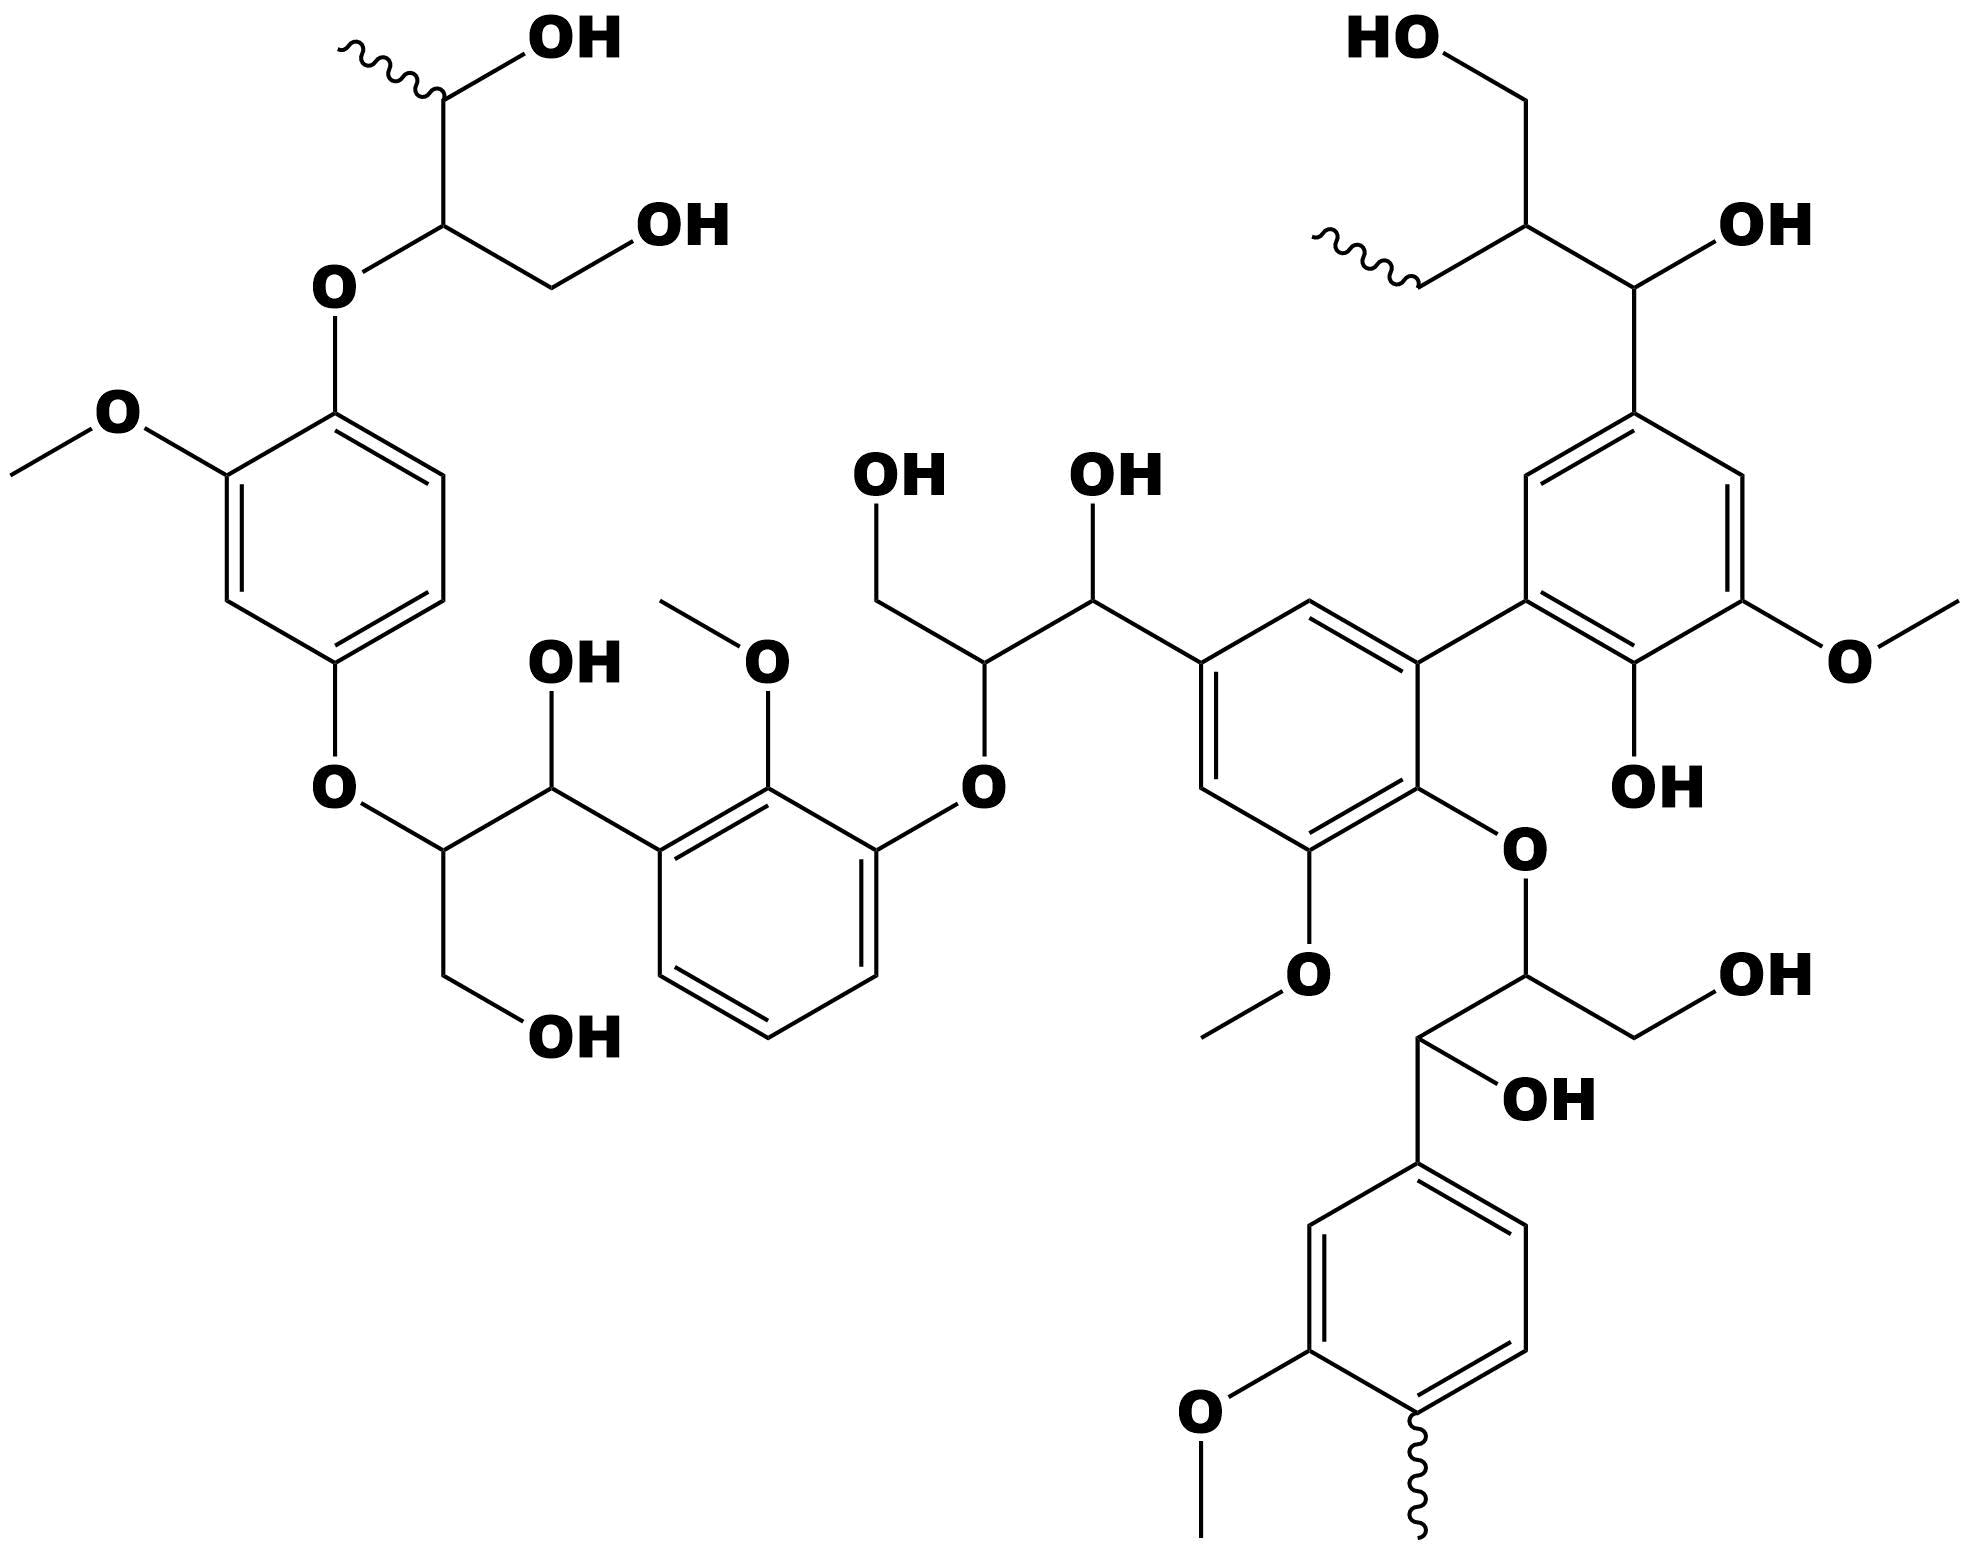
\includegraphics[width=0.5\textwidth]{SF/lignin}
    %\caption{Structure of Lignin- The lignin content of hemp will vary according to the part of the plant under observation. It contains a number of carbonyl, ester groups along with other proteins such as edestin and albumin.}
  %\label{SF:lignin}
%\end{figure}
%\begin{figure}[tbh!]
  %\centering
  %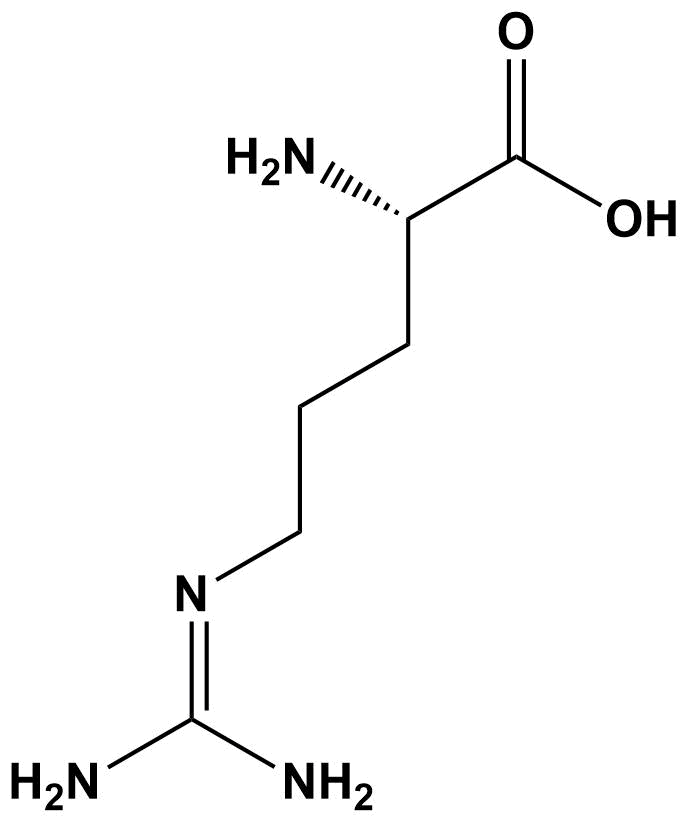
\includegraphics[width=0.5\textwidth]{SF/arginine}    \caption{Structure of Arginine- major component of hemp fibers containing C-N, C=O, C-O bonds.}
  %\label{SF:arginine}
%\end{figure}
%\begin{figure}[tbh!]
  %\centering
  %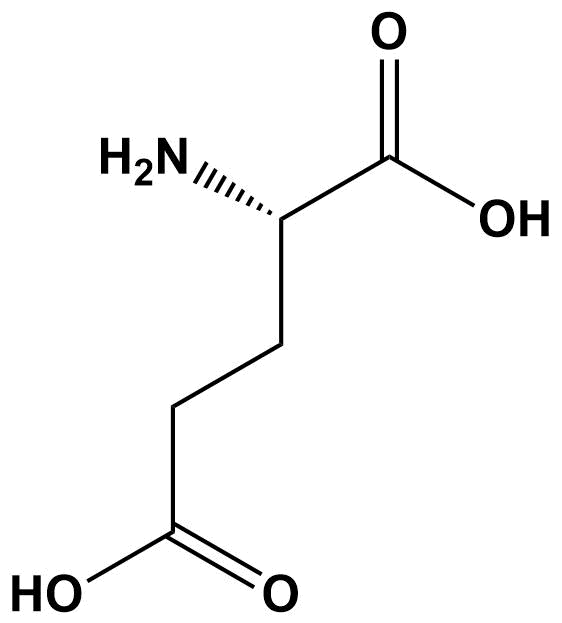
\includegraphics[width=0.5\textwidth]{SF/glutamicacid}
    %\caption{Structure of Glutamic acid- another protein found in hemp fibers containing C-O, C=O and C-N bonds.}
  %\label{SF:glutamicacid}
%\end{figure}
\begin{figure}[th!]
\centering
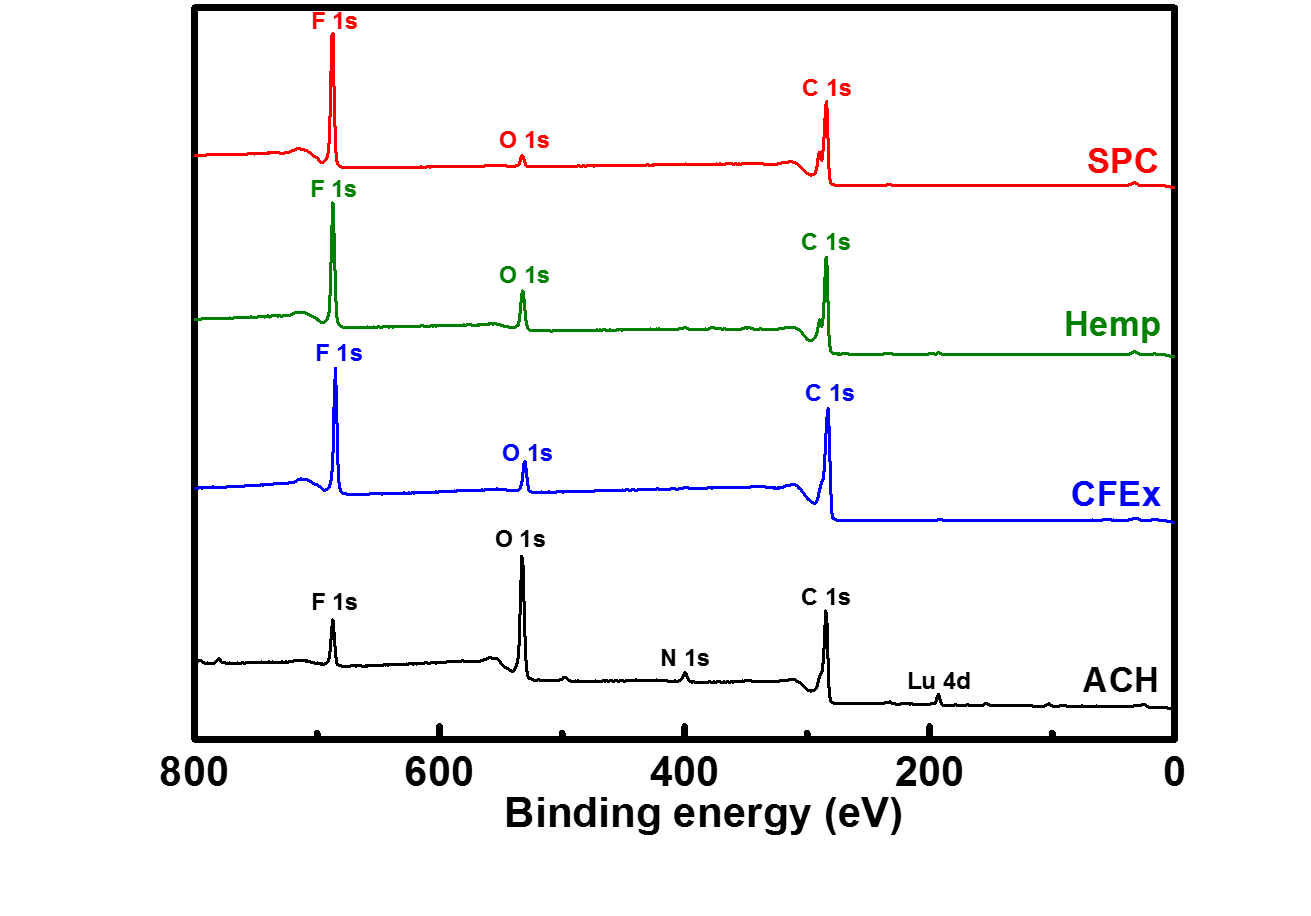
\includegraphics[width=\textwidth]{fig/XPSoverall}
\caption{Overall spectra of ACH (blck), hemp fibers (blue), CFEx (green) and SUper-P(red).}
\label{fig:XPSoverall}
\end{figure}

\begin{figure}[th!]
\centering

\includegraphics[width=\textwidth]{fig/hair50mVs}
\caption{Cyclic voltammogram of ACH at a scan rate of 50 mV/s in a two electrode setup against \ce{Al3+}/Al showing a capacitor-like behaviour with no visible oxidation-reduction peaks unlike Figure \ref{fig:CV}b where we distinctly observed redox peaks.}
\label{fig:hair50mVs}
\end{figure}

\begin{figure}[th!]
\centering
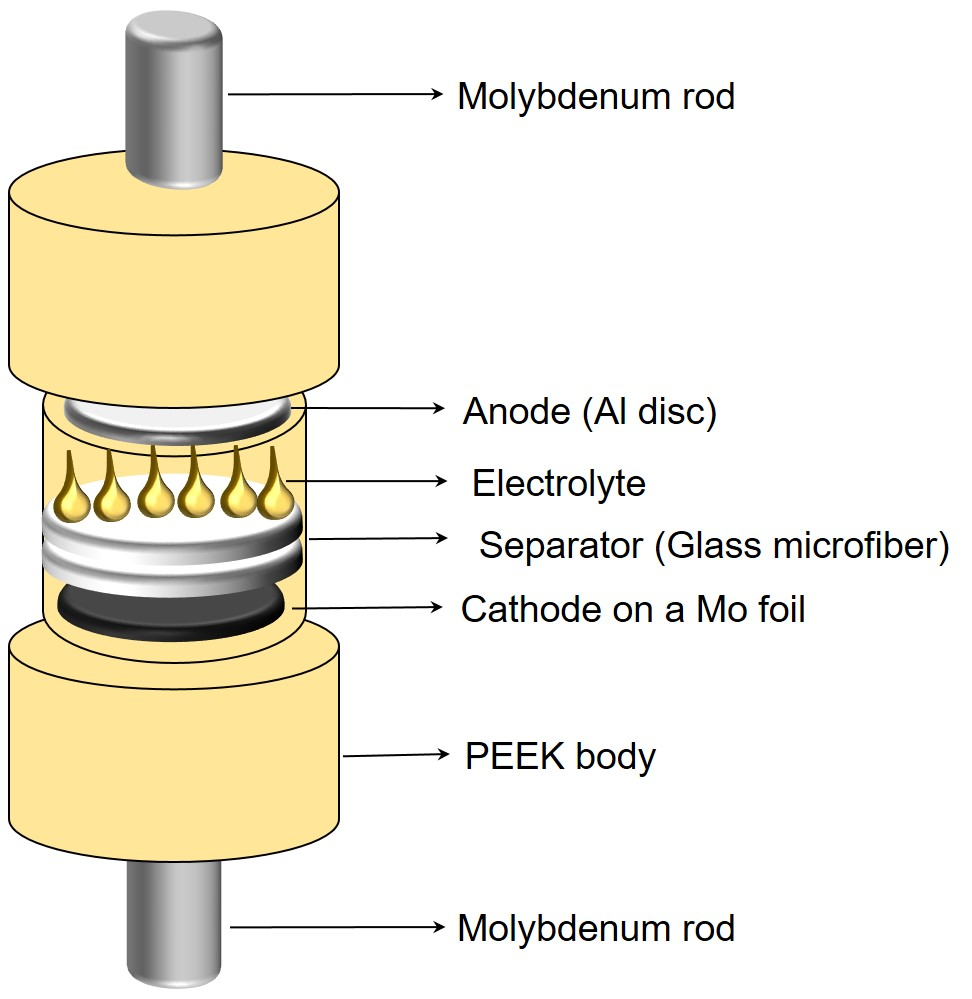
\includegraphics[width=\textwidth]{fig/PEEK}
\caption{A custom-made two-electrode polyetherether ketone (PEEK) cell used for galvanostatic cycles and cyclic voltammetry.}
\label{fig:PEEK}
\end{figure}

\end{document}